In order to fulfill the objectives described in Section~\ref{objectives}, a convenient and dynamic methodology should be implemented.

Given the great deal of software development, reverse engineering and debugging involved in the specific objectives, it is required to build a research plan with a methodology able to: 
\begin{itemize}
	\item Adapt to constant changes in the specific objectives/phases, even at advanced stages.
	\item Consider collaboration with peers acquainted with other knowledge areas.
	\item Facilitate frequent working-software deliveries with minimum bugs.
\end{itemize}

Based on this, it is thought to implement the principles of Agile Software Development~\cite{agileAlliance,agileManifesto}, which very well correspond with the requirements mentioned above.

\subsection{Short-term Control}\label{shot-termContol}
Following the recommendations provided by the Agile methodology, a fifteen-minute meeting will be held everyday (if possible) with the thesis supervisor. This short, and preferably standing-up meetings complement the process of development by:

\begin{itemize}
	\item Helps in keeping everyone up-to-date on the state of the development.
	\item Increases supervisor-student collaboration.
	\item Helps keep the high frequency of the technical reports.
\end{itemize}

These technical reports are to be delivered on a monthly basis and must provide sufficient overview of the research efforts, including:

\begin{itemize}
	\item Current state of the research (looking at the objectives/phases).
	\item Past, current and future tasks (up until the next report).
	\item Required knowledge or material to fulfill the current objective/phases.
\end{itemize}

By implementing the Agile recommendations and following the short-term control measures described above, it is possible to keep track of the efforts towards the general objective.

\subsection{Description of the Plan by Years}\label{planByYears}
Agile methods are thought to be adaptive, meaning that the far future (six months from now) will present unknown problems; nevertheless it is more efficient at solving short-term problems, as was described previously at Section~\ref{shot-termContol}.

To leverage this issue, the objectives presented in Section~\ref{objectives} can be distributed over the remaining years as follows:

\begin{itemize}
	\item {\bfseries First year:} at the time of this writing, objectives~\ref{ECAHysteresis},~\ref{incorporateECA},~\ref{metrics},~\ref{scenarios} are either finished or ongoing work. Further details can encountered at Section~\ref{priorWork}. The remaining phases of the first specific objective are to be finished during the first year.
	\item {\bfseries Second year:} will be dedicated to the study of the WMP architecture. This step will provide the knowledge to continue achieving objectives. It is expected to achieve specific objective~\ref{learningWMP}, as well as~\ref{WMPModifications} and~\ref{accessByteCode}.
	\item {\bfseries Third year:} is to be dedicated at the completion of specific objective~\ref{ECAinWMP} and~\ref{ECAinRFID}.
\end{itemize}

A summary of the distribution of the activities throughout the remaining years is shown in Figure~\ref{fig:gantt}.

\begin{figure}[htbp]
  \centering
  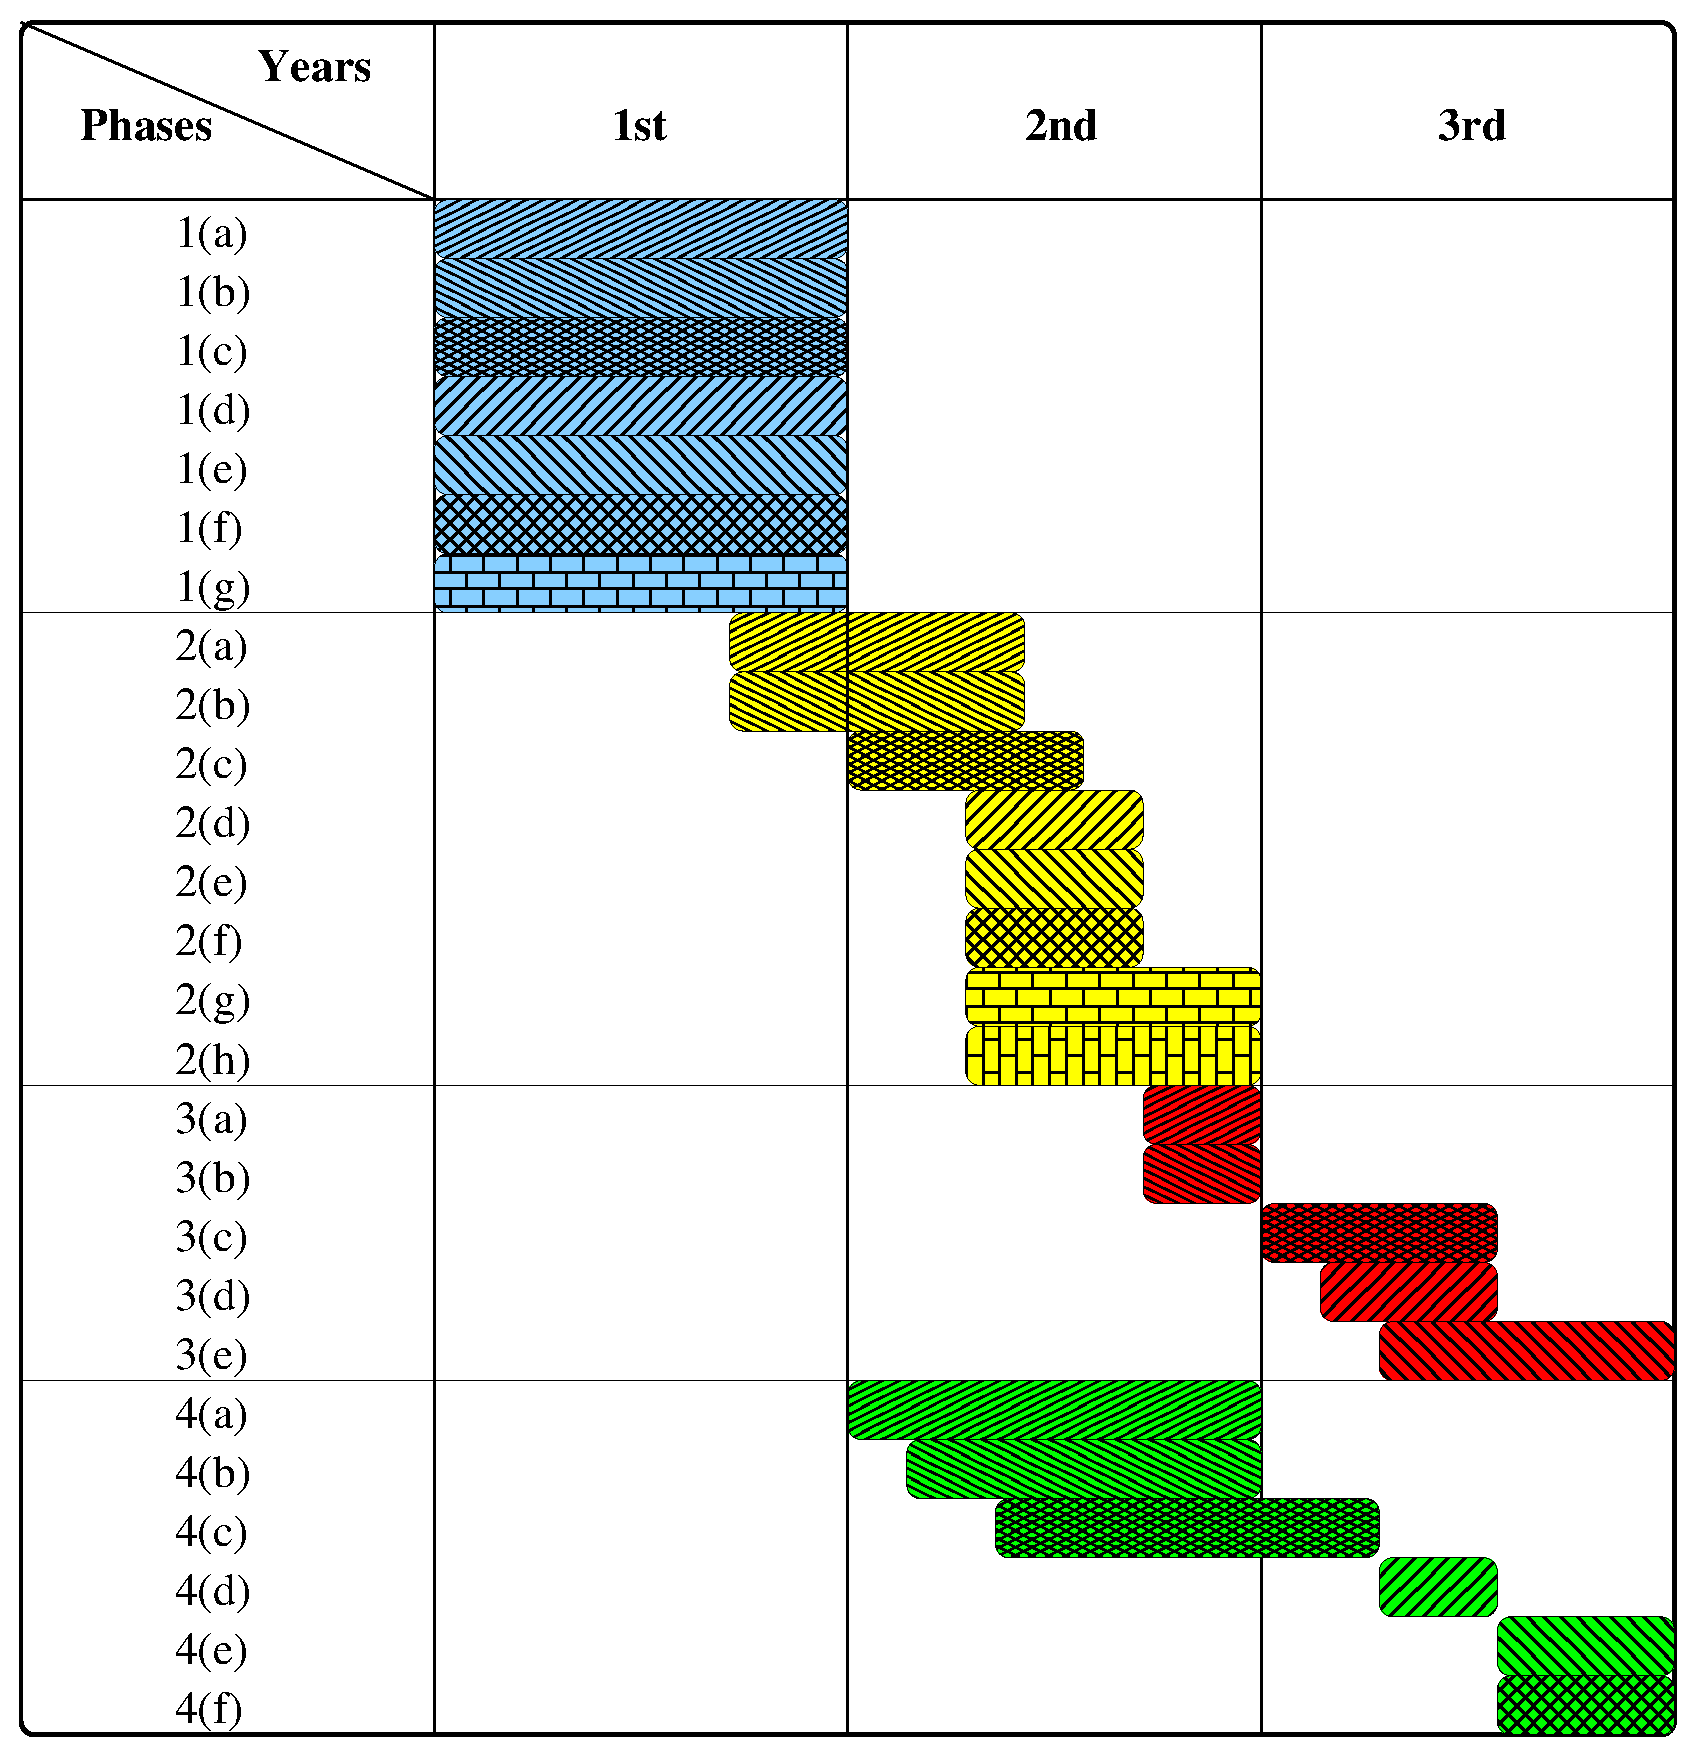
\includegraphics[width=\linewidth]{gantt.eps}
  \caption{Gantt diagram
  \label{fig:gantt}}
\end{figure}